\chapter{Numerical methods}

% ==================================================================================================

\section{Motivation}
There are numerous reasons why we may want to solve equations. For instance, we may want to find the roots of a function $f$, i.e. the values of $x$ that satisfy $f(x) = 0$. In the case of quadratic equations in the general form $ax ^ 2 + bx + c = 0$, the roots are given by the quadratic formula
\[
  x = \frac{-b \pm \sqrt{b ^ 2 - 4ac}}{2a}
\]
However, it is not always this easy to find the roots of any arbitrary function, or solve any arbitrary equation. In fact, we may not always be able to find analytic solutions to equations. Our next best bet would be approximating the values of the solutions. The tools that allow us to approximate \textit{numerical} values of solutions are called \textit{numerical methods}.

% ==================================================================================================

\section{Newton-Raphson method}
The Newton-Raphson method allows us to approximate the roots of a given function.

% --------------------------------------------------------------------------------------------------

\subsection{How it works}
\begin{figure}[!htbp]
  \centering
  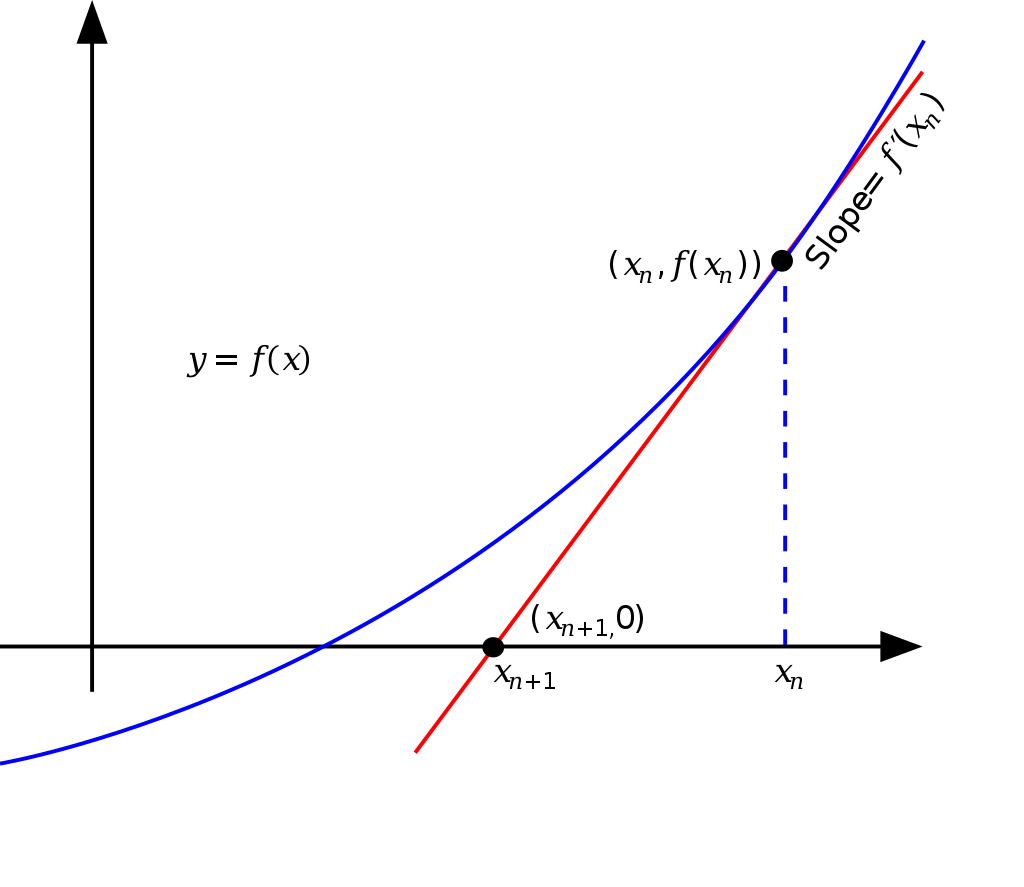
\includegraphics[width=0.6\columnwidth]{week_08_newton}
  \caption{Newton-Raphson method}
\end{figure}
Consider a differentiable (and hence continuous) function $f$. We pick an initial guess $x_0$. Then, we calculate the $x$-intercept of the tangent line to the curve $y = f(x)$ at $x_0$ to obtain $x_1$. We keep iterating this process until we are satisfied. This could mean either:
\begin{itemize}
  \item We have performed sufficiently many iterations, or
  \item The result is close enough to the root, i.e. $f(x)$ is close enough to $0$ (since $f$ is continuous).
\end{itemize}
\begin{definition}[Newton-Raphson]
  \label{def:newton-raphson}
  Given an approximation $x_n$, the next approximation $x_{n + 1}$ is given by
  \[
    x_{n + 1} = x_n - \frac{f(x_n)}{f'(x_n)}
  \]
\end{definition}

% --------------------------------------------------------------------------------------------------

\subsection{Derivation}
Given some approximation of the root $x_n$, we define the next approximation $x_{n + 1}$ to be the $x$-intercept of the tangent line passing through $f(x_n)$. Recall that the equation of this tangent line is
\begin{equation}
  y = f(x_n) + f'(x_n) (x - x_n)
  \label{eqn:newton-raphson-tangent}
\end{equation}
\begin{intuition}
  The slope of any line is defined to be \textit{rise over run}, so the difference in $y$-coordinate (\textit{rise}) is equal to the slope times the \textit{run} ($x - x_n$). This difference is relative to the $y$-coordinate we started with, which is $f(x_n)$.

  Alternatively, we can derive this from the definition of slope:
  \[
    f'(x_n) = \frac{y - f(x_n)}{x - x_n}
  \]
\end{intuition}
Substituting $(x, y) = (x_{n + 1}, 0)$ into \Cref{eqn:newton-raphson-tangent}, we get
\begin{equation}
  0 = f(x_n) + f'(x_n) (x_{n + 1} - x_n)
  \label{eqn:newton-raphson-x_n+1}
\end{equation}
and a little bit of rearranging gives us
\[
  x_{n + 1} = x_n - \frac{f(x_n)}{f'(x_n)}
\]
Since we have $f'(x_n)$ in the denominator, we must have that $f'(x_n) \neq 0$.

% --------------------------------------------------------------------------------------------------

\subsection{Order of convergence}
We might want to know how fast the Newton-Raphson method can give us a \textit{good enough} approximation to a root of the function. An approximation $x$ is \textit{good enough} if it is within some predefined value $\epsilon$ of the root $r$, so $\abs{x - r} \leq \epsilon$. We define $\epsilon_n = \abs{x_n - r}$. (In other literature, there are no absolute value bars.)

Let $f$ be a function with a continuous second derivative. Then by Taylor's theorem, we can express $f(x)$ as a 1st order Taylor polynomial centred at $x_n$:
\[
  f(x) = f(x_n) + f'(x_n) (x - x_n) + \frac{1}{2} f''(c) (x - x_n) ^ 2
\]
for some $c$ between $x$ and $x_n$. We set $x = r$ to get
\[
  f(r) = f(x_n) + f'(x_n) (r - x_n) + \frac{1}{2} f''(c) (r - x_n) ^ 2
\]
for some $c$ between $x_n$ and $r$. Since $r$ is a root, by definition, $f(r) = 0$. So
\begin{equation}
  0 = f(x_n) + f'(x_n) (r - x_n) + \frac{1}{2} f''(c) (r - x_n) ^ 2
  \label{eqn:newton-raphson-taylor}
\end{equation}
Subtracting \Cref{eqn:newton-raphson-x_n+1} from \Cref{eqn:newton-raphson-taylor} gives us
\[
  0 = f'(x_n) (r - x_{n + 1}) + \frac{1}{2} f''(c) (r - x_n) ^ 2
\]
Rearrange the equation a little bit to get
\[
  x_{n + 1} - r = \frac{f''(c)}{2f'(x_n)} (x_n - r) ^ 2
\]
Taking the absolute value of both sides, we get
\begin{align*}
  \abs{x_{n + 1} - r} &= \frac{\abs{f''(c)}}{2\abs{f'(x_n)}} \abs{x_n - r} ^ 2 \\ 
  \epsilon_{n + 1} &= \frac{\abs{f''(c)}}{2\abs{f'(x_n)}} \epsilon_n ^ 2
\end{align*}
From this result, we say that the Newton-Raphson method has \textbf{quadratic convergence}. However, certain conditions have to be satisfied:
\begin{theorem}
  The Newton-Raphson method has at least quadratic convergence if the following conditions are satisfied:
  \begin{enumerate}
    \item $f'(x) \neq 0$ for every $x \in I \coloneqq [r - \epsilon_0, r + \epsilon_0]$
    \item $f''$ is continuous on $I$---this is the assumption for Taylor's theorem.
    \item $M\epsilon_0$ < 1, where $M$ is defined to be
      \[
        M = \frac{1}{2} \left(\sup_{x \in I} \abs{f''(x)}\right) \left(\sup_{x \in I} \frac{1}{\abs{f'(x)}}\right) 
      \]
  \end{enumerate}
\end{theorem}
\begin{remark}
  A few notes on the third condition:
  \begin{itemize}
    \item The supremum is attained because $f$ is continuous (since $f'$ exists), so it is the global maximum of $f$ restricted to $I$.
    \item We must take the suprema separately, as opposed to something like
      \[
        \sup_{x \in I} \frac{\abs{f''(x)}}{2\abs{f'(x)}}
      \]
      since the $x$ in the numerator is some unknown value $c$ between $x_n$ and $r$, as determined by Taylor's theorem, while the $x$ in the denominator is our guess $x_n \neq c$.
    \item We specify $M\epsilon_0 < 1$ because we want $\epsilon_n$ for all $n \geq 1$ to be no larger than $\epsilon_0$, so that all of our subsequent approximations will be within $I$ (hence $I$ is defined as such):
      \[
        \epsilon_1 = \frac{\abs{f''(c)}}{2\abs{f'(x)}} \epsilon_0 ^ 2 < 1 \times \epsilon_0 = \epsilon_0
      \]
      It follows by induction that
      \[
        \epsilon_n \leq M ^ {2n - 1} \epsilon_0 ^ {2n} = \frac{1}{M} (M\epsilon_0) ^ {2n}
      \]
      By the squeeze theorem, $\epsilon_n$ converges to 0 (i.e. the approximations get arbitrarily close to the root) if $M\epsilon_0 < 1$.
  \end{itemize}
\end{remark}

% --------------------------------------------------------------------------------------------------

\subsection{Limitations}
Some of the limitations of the Newton-Raphson method are outlined in \Cref{tab:newton-raphson-limitations}.
\begin{table}[!htbp]
  \centering
  \ra{1.2}
  \caption{Limitations of the Newton-Raphson method}
  \label{tab:newton-raphson-limitations}
  \begin{tblr}{colspec = {X[2, c, m] X[4, h, c] X[2, c, m]}, rowhead = 1, row{1} = {font = \bfseries}}
    \toprule
    \multicolumn{1}{c}{\textbf{Limitation}} & \multicolumn{1}{c}{\textbf{Example}} & \multicolumn{1}{c}{\textbf{Workaround}} \\ 
    \midrule
    The function is not differentiable. & {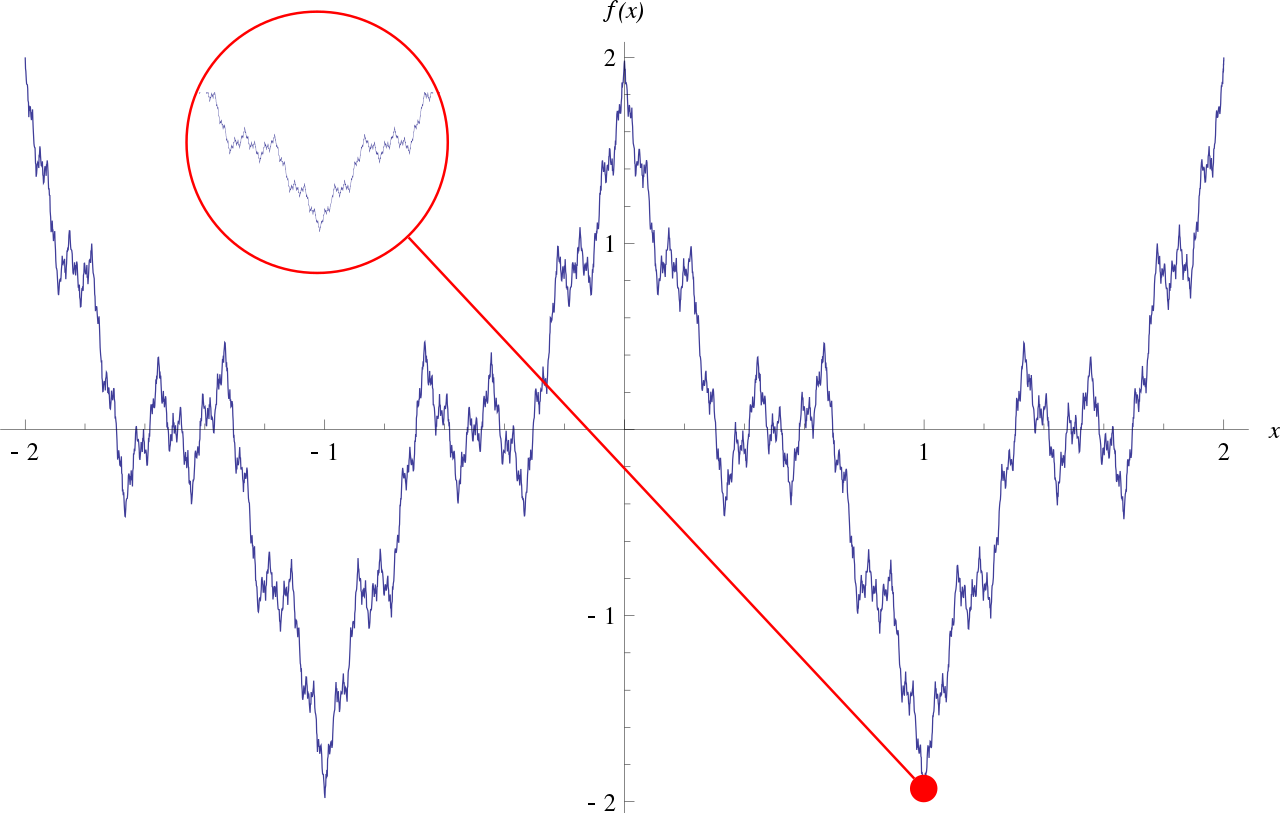
\includegraphics[width=0.3\textwidth]{week_08_newton_weierstrass_function} \\ The Weierstrass function is continuous but not differentiable.} & Use the secant method instead. \\
    \midrule
    Tangent lines keep oscillating. & {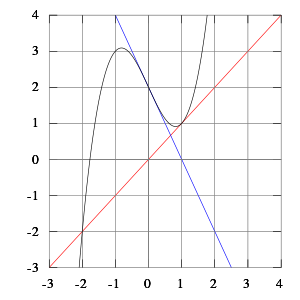
\includegraphics[width=0.3\textwidth]{week_08_newton_fail} \\ When applied to the function $y = x ^ 3 - 2x + 2$, Newton's method oscillates between $0$ and $1$.} & Pick a different starting point, perhaps using the bisection method. \\ 
    \midrule
    Diverges. & {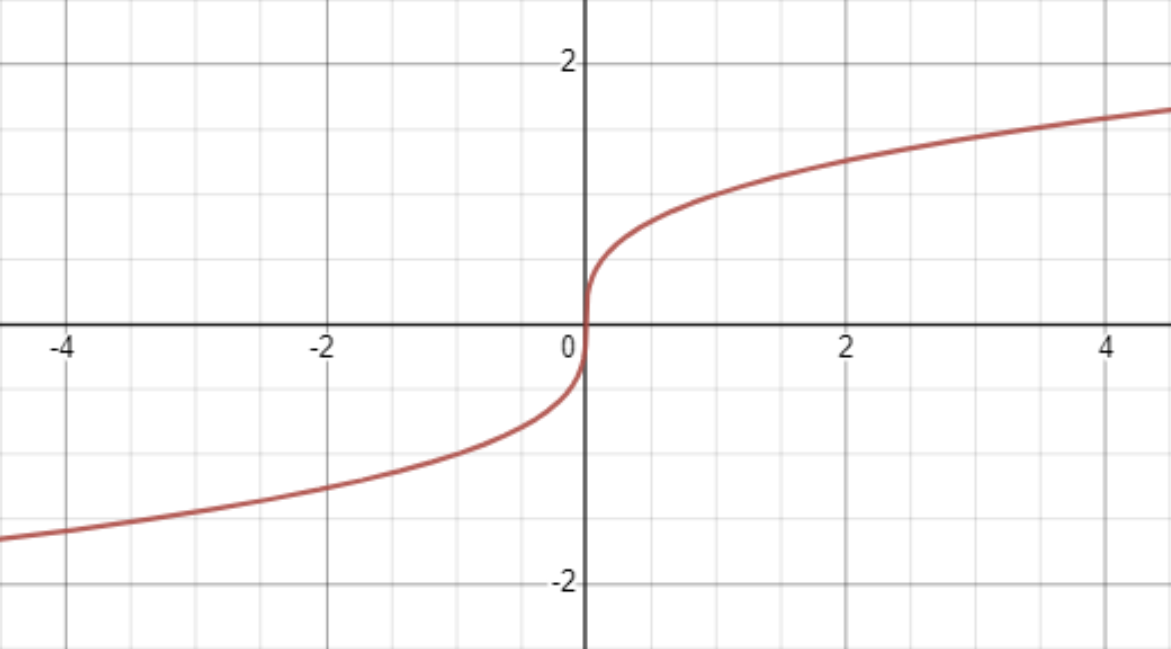
\includegraphics[width=0.3\textwidth]{week_08_newton_diverges} \\ Consider the function $f(x) = \sqrt[3]{x}$. \\ $ x_{n + 1} = x_n - \dfrac{x_n ^ {1 / 3}}{\frac{1}{3} x_n ^ {-2 / 3}} = -2x_n $ \\ which diverges for all $x_n \neq 0$. But then $f'(0)$ is undefined.} & RIP. \\
    \bottomrule
  \end{tblr}
\end{table}

% ==================================================================================================

\section{Quasi-Newton methods: secant method}
In the Newton-Raphson method, we computed the first derivative at every approximation to find the next approximation. However, computing derivatives may be expensive. Instead, we may use an approximation for the derivative. Numerical methods that approximate the derivative instead of computing its precise value are called \textit{quasi-Newton methods}. One such method is the secant method.

% --------------------------------------------------------------------------------------------------

\subsection{How it works}
\begin{figure}[!htbp]
  \centering
  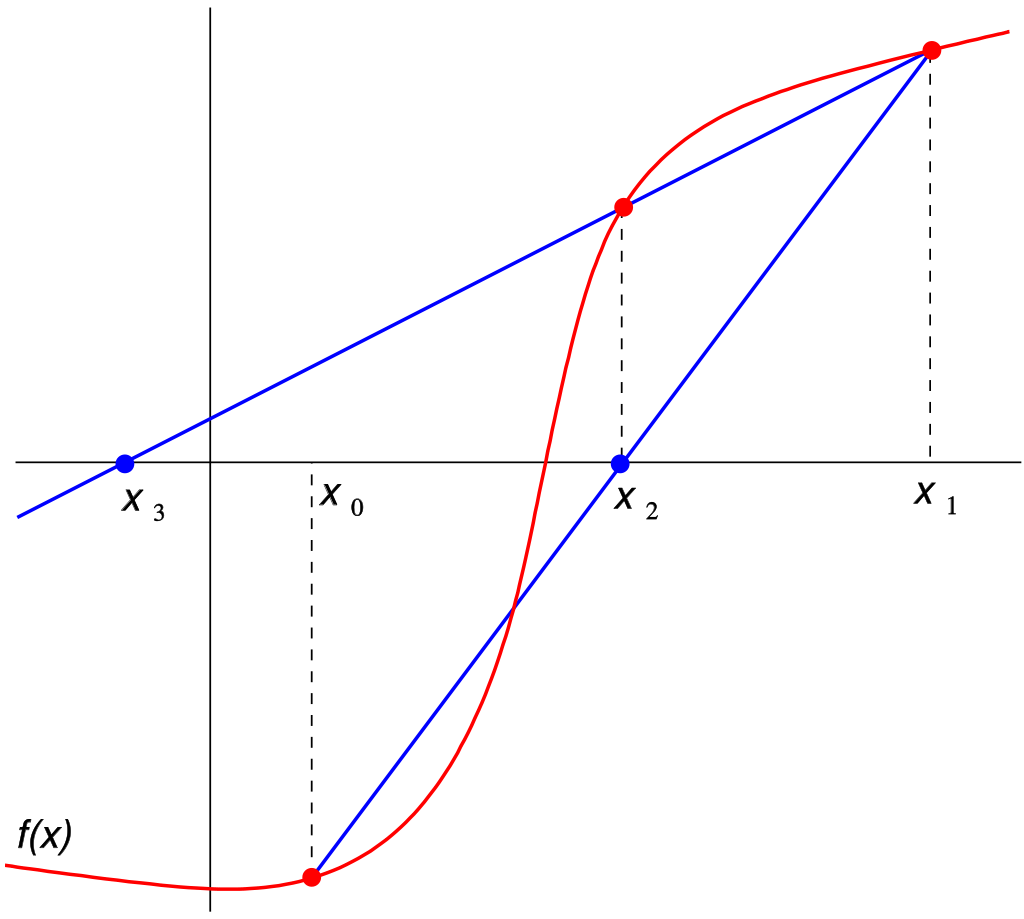
\includegraphics[width=0.6\columnwidth]{week_08_secant}
  \caption{Secant method}
\end{figure}
Suppose we want to find the roots of a function $f$. We pick two initial guesses $x_0$ and $x_1$, and draw the secant passing through the two points $(x_0, f(x_0))$ and $(x_1, f(x_1))$. Our next approximation $x_2$ is the $x$-intercept of this secant line. We keep drawing the secant lines using our two most recent guesses until satisfied.
\begin{definition}[Secant method]
  Given the two most recent approximations $x_n$ and $x_{n - 1}$, the next approximation $x_{n + 1}$ is given by
  \[
    x_{n + 1} = x_n - f(x_n) \frac{x_n - x_{n - 1}}{f(x_n) - f(x_{n - 1})}
  \]
\end{definition}
\begin{intuition}
  We approximate the tangent line by the secant line, so
  \[
    f'(x_n) \approx \frac{f(x_n) - f(x_{n - 1})}{x_n - x_{n - 1}}
  \]
  Substituting this into \Cref{def:newton-raphson} and replacing the approximation with equality gives us the required form.
\end{intuition}

% --------------------------------------------------------------------------------------------------

\subsection{Derivation}
The equation of the secant line between $(x_n, f(x_n))$ and $(x_{n - 1}, f(x_{n - 1}))$ is given by
\begin{equation}
  y = f(x_n) + (x - x_n) \frac{f(x_n) - f(x_{n - 1})}{x_n - x_{n - 1}}
  \label{eqn:secant}
\end{equation}
Substituting $(x, y) = (x_{n + 1}, 0)$ into \Cref{eqn:secant} gives us
\[
  0 = f(x_n) + (x_{n + 1} - x_n) \frac{f(x_n) - f(x_{n - 1})}{x_n - x_{n - 1}}
\]
and a little bit of rearranging turns this into
\[
  x_{n + 1} = x_n - f(x_n) \frac{x_n - x_{n - 1}}{f(x_n) - f(x_{n - 1})}
\]

% --------------------------------------------------------------------------------------------------

\subsection{Order of convergence}
The secant method bears the advantage of lower computational costs, as it does not require computing derivatives. With this advantage comes a disadvantage: the secant method converges to a root slower than the Newton-Raphson method. In fact, the order of convergence is the golden ratio
\[
  \frac{1 + \sqrt{5}}{2}
\]
but we will not go into the derivation here.

% ==================================================================================================

\section{Initial value problem}
An initial value problem is a differential equation
\[
  \frac{\di y}{\di t} = f(t, y)
\]
given the initial conditions $(t_0, y_0)$. Solutions to initial value problems are, of course, functions, but sometimes we may only want to know the value of a solution function $y$ evaluated at a certain point $t_n$. The following methods allow us to generate a sequence of approximations at $t_1, t_2, \ldots$.

% --------------------------------------------------------------------------------------------------

\subsection{Euler's method}
In Euler's method, we approximate the solution curve by tangent lines. Given $t_0$ and $y_0$, suppose we want to approximate the solution at $t_1$. The tangent line passing through $(t_0, y_0)$ has the equation
\[
  y = y_0 + f(t_0, y_0) (t - t_0)
\]
since $f(t_0, y_0)$ is given to be the slope of the tangent line at $t_0$. Setting $(t, y) = (t_1, y_1)$ gives us
\[
  y_1 = y_0 + f(t_0, y_0) (t_1 - t_0)
\]
In general,
\begin{definition}[Euler's method]
  Given $t_n$ and the approximation of the solution at this point $y_n$, the next approximation at $t_{n + 1}$ is given by
  \[
    y_{n + 1} = y_n + f(t_n, y_n) (t_{n + 1} - t_n)
  \]
\end{definition}
Sometimes, we may want to use a uniform step size, i.e. for every $n$, $t_{n + 1} - t_n = h$ for some $h$. Then we can rewrite Euler's method as
\[
  y_{n + 1} = y_n + hf(t_n, y_n)
\]
Notice we can also neatly express $t_n$ in terms of $h$ and $t_0$:
\[
  t_n = t_0 + hn
\]
% --------------------------------------------------------------------------------------------------

\subsection{Modified Euler's method (Heun's method)}
The improved Euler's method, also known as Heun's method, is the simplest example of a \textit{predictor-corrector method}. Heun's method \textit{corrects} some of the error in Euler's method by taking the average of the slopes at $(t_n, y_n)$ and $(t_{n + 1}, y_{n + 1}^*)$, where $y_{n + 1}^*$ denotes the approximation at $x_{n + 1}$ using Euler's method:
\[
  y_{n + 1}^* = y_n + hf(t_n, y_n)
\]
We state this mathematically.
\begin{definition}[Heun's method]
  Given $t_n$ and the approximation of the solution at this point $y_n$, the next approximation at $t_{n + 1}$ is given by
  \[
    y_{n + 1} = y_n + \frac{1}{2} (f(x_n, y_n) + f(x_{n + 1}, y_{n + 1}^*))h
  \]
\end{definition}

% --------------------------------------------------------------------------------------------------

\subsection{Runge-Kutta method}
The Runge-Kutta method is another example of a predictor-corrector method. It takes the weighted average of four slopes:
\begin{definition}[Runge-Kutta method]
  Given $t_n$ and the approximation of the solution at this point $y_n$, the next approximation at $t_{n + 1}$ is given by
  \[
    y_{n + 1} = y_n + \frac{1}{6}(k_1 + 2k_2 + 2k_3 + k_4) h
  \]
  where
  \begin{itemize}
    \item $k_1 = f(t_n, y_n)$---the slope at $t_n$
    \item $k_2 = f(t_n + \frac{h}{2}, y_n + \frac{h}{2} k_1)$---the slope halfway between $t_n$ and $t_{n + 1}$
    \item $k_3 = f(t_n + \frac{h}{2}, y_n + \frac{h}{2} k_2)$---the slope halfway between $t_n$ and $t_{n + 1}$, this time using $k_2$
    \item $k_4 = f(t_n + h, y_n + hk_3)$---the slope at $t_{n + 1}$
  \end{itemize}
\end{definition}